 \begin{wrapfigure}[0]{r}[-1cm]{1cm}
   \vspace{-6cm}
   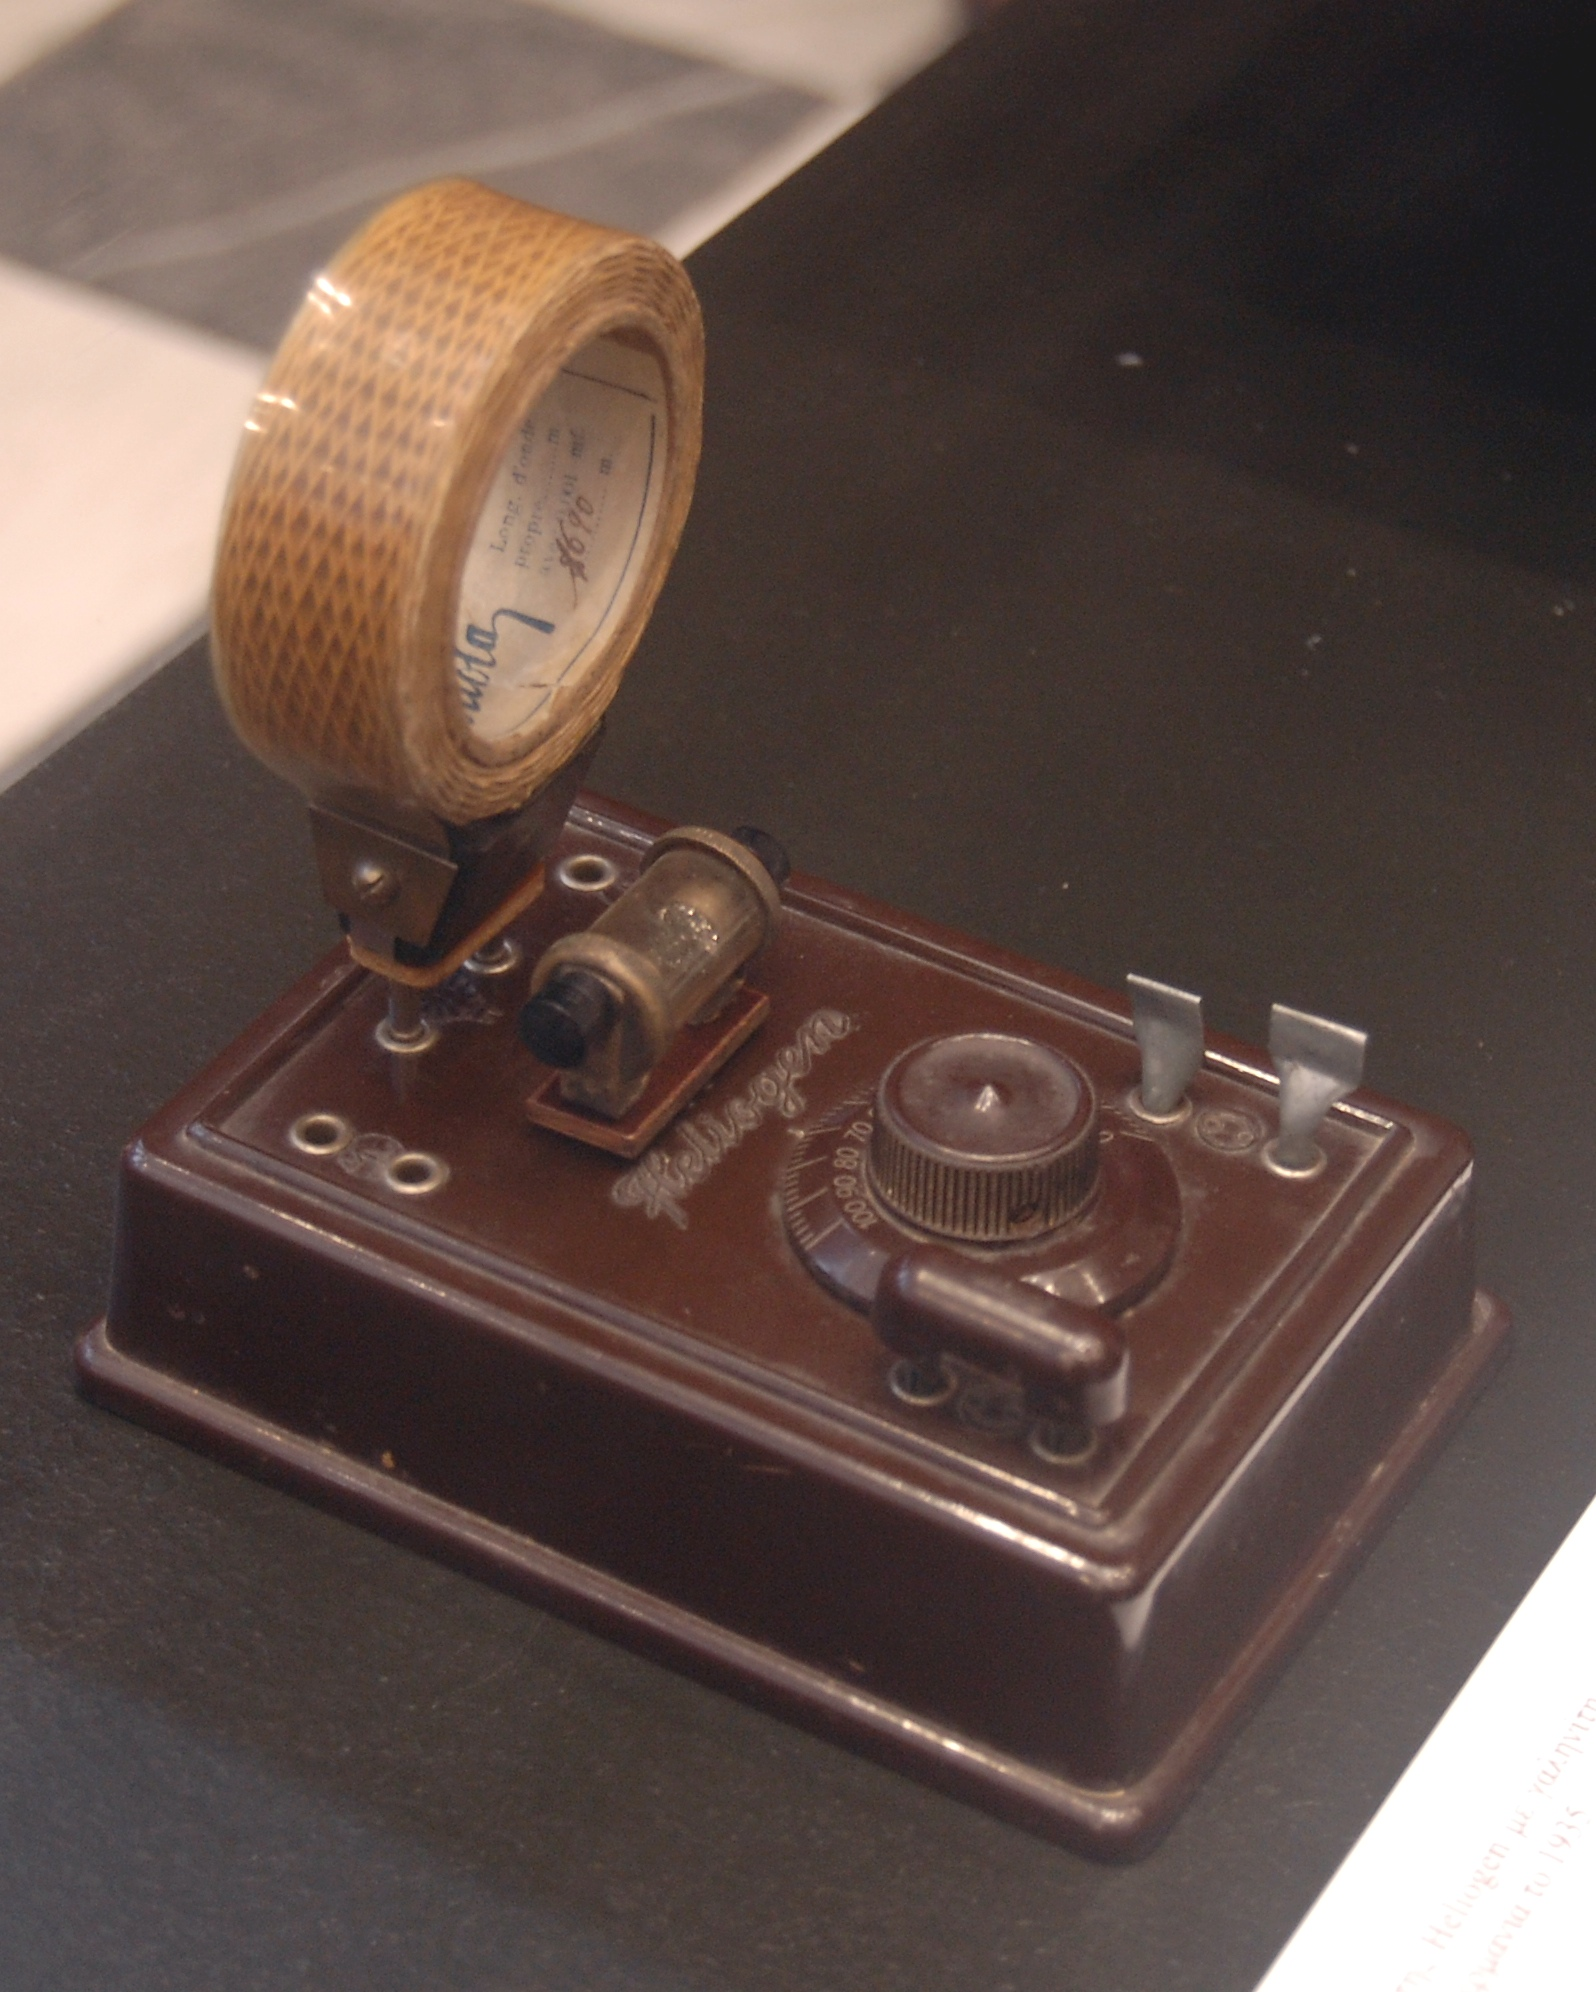
\includegraphics[scale=0.07]{Kurzwellendetektor/Bilder/Heliogen_medium_wave_galena_radio.JPG}
  \vspace{-6cm}
 \end{wrapfigure}

\section*{Praktische Anwendung}

\loesung{Mit den Lautsprechern funktioniert es ganz gut. Ggf. können sich die
SWL Kopfhörer mitbringen und diese mit einem Klinkenbuchsenadapter direkt
``anstöpseln.''

Mit der Spule um die $2.5 \mu H$ und dem DrehKo um die $200 pF$ befindet man
sich irgendwo im 40m-Band. Da Kurse meist Nachmittags/Abends stattfinden, bietet
sich dieses Band an. Für schnelle Erfolge kann man einen TRX mitnehmen und auf
dem Band in AM senden.

}

Radio- und Funk-Signale empfangen ohne die Verwendung einer Batterie oder einer
anderen Energiequelle? Eine einfache Schaltung ermöglicht das. Die folgende
Schaltung eines Detektorempfängers ist die einfachste aller Radioschaltungen. In
der Frühzeit der Radiotechnik war das Konzept eines Detektorempfänger durchaus
verbreitet, da es den Rundfunkempfang mit wenigen Bauteilen ermöglichst. Heute
ist es leider nich mehr ohne weiters möglich Radio-Sendungen mit dem der
Kurzwellendetektor zu empfangen, da der Großteil der Kurz- und
Mittelwellensender ihren Betrieb eingestellt haben. Nichts desto trotz ist er
ein guter Einstieg und ein technisches Abenteuer.

\begin{enumerate}
    %\itemsep1pt\parskip0pt\parsep0pt
  \item Berechnet die minimale und maximale Frequenz eines Schwingkreis mit
    eurer Spule (ggf. nochmal mit dem LC-Meter nachmessen) und einem
    Plattenpaket des DrehKos. Die minimal einstellbare Kapazität liegt bei ca.
    $5 pF$. Welche Afu-Bänder liegen in dem Bereich?  \loesung{Bei einer Spule
    um die $2.5 uH$ ist der Schwingkreis zwischen ca. 6 und 45 MHz tunebar.
    Bänder: Alle KW-Bänder ab 40m bis 10m.}
  \item Baue die Schaltung aus Abbildung \ref{kd} mit der bereits gebauten
    Spule und einem so genannten Langdraht als Antenne auf -- die länge der
    Antenne ist für den Empfang erstmal nicht so relevant. Bei dem
    eigentlichen "`Detektor"' handelt es sich um eine Germaniumdiode (z.B. AA
    143). Etwas weniger gut, aber weitaus preiswerter ist die Verwendung einer
    Schottky-Diode (z.B. BAT 43).  Was könnte die Diode tun und warum
    verwendet man keine Si-Dioden?
    \loesung{Dies ist ein Vorgriff auf die AM-Modulation. Die Diode
    demoduliert je nach Polung die obere oder untere Einhüllende.
    Germanium/Schottky-Dioden haben eine Schwellenspannung von ca. $0.3 V$,
    Silizium-Dioden arbeiten erst ab $0.6 V$ bis $0.7 V$.}
  \item Abgestimmt wird der Detektor mit dem DrehKo (gegen den Uhrzeigersinn
    gedreht wird die Kapazität größer). Mit diesem einfachen Aufbau können nur
    wirklich starke Sender empfangen werden -- wir simulieren das mit einem
    Funkgerät.  Mit etwas Glück kann aber auch ein echter Sender empfangen
    werden.
  \item Verwende den zuvor gebauten Audio-Verstärker, um empfangene Signale
    besser hörbar zu machen.
  \item Messt mit Hilfe des LC-Meters euren DrehKo aus und berechnet den
    Schwingkreis. In welchem Band werden die Signale der Antenne empfangen?
    \loesung{Die Spule hat um die $2.5 uH$ und der DrehKo max. $265 pF$ Die SWL
    sollen das schön per Hand rechnen. Zum Nachprüfen kann man z.B. dieses Tool
    verwenden: \url{http://wetec.vrok.de/rechner/cskreis.htm}}
\end{enumerate}

% TODO Kann man den Empfang mit einem anderen Spulenanzapf verbessern?

\begin{figure}[H]
    \centering
    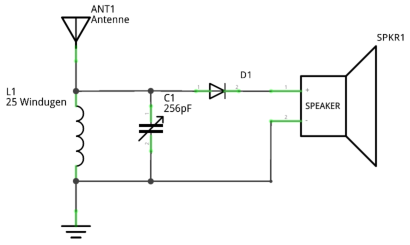
\includegraphics[scale=0.9]{Kurzwellendetektor/Bilder/Kurzwellendetektor_Schaltplan.pdf}
    \caption{Der Kurzwellendetektor}
    \label{kd}
\end{figure}
